\documentclass[
  dvipdfmx
]{standalone}
\usepackage{tikz}
\usetikzlibrary{spath3}
\usetikzlibrary{knots}
\usetikzlibrary{hobby}
\usetikzlibrary{patterns}
\begin{document}
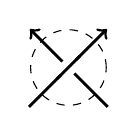
\begin{tikzpicture}
  \begin{knot}[
    consider self intersections=true,
    ignore endpoint intersections=false,
    every strand/.append style={line width=1pt},
    clip width=6,
    clip radius=4pt,
    flip crossing=1,
    % background color=red,
  ]
  \strand[->] (1,0) -- (0,1);
  \strand[->] (0,0) -- (1,1);
  \end{knot}
  \draw[dashed] (0.5,0.5) circle[radius=0.48];
\end{tikzpicture}
\end{document}